\chapter{Implementation of Dynamic Graph Tracking in Julia}
\label{cha:impl-dynam-graph}

It has been mentioned above that there is a trade-off between source-transformation methods and
library-based approaches for tracking computation graphs.  Since the ultimate goal of this work was
to analyze dynamic probabilistic models written in \turingjl{}, properties of both were derired.
Inspired the the work of \textcite{innes2018don}, it seemed most promising to start from a
source-transformation based approach implemented over the intermediate representation, especially
from a usability point of view.  The advantages of using IR over the surface AST are the same: there
is less overhead from handling multiple syntactic forms, and naming is already referentially
transparent.  Additionally, there are existing Julia packages to simplify handling the IR data
structures and set up the transformations.\todo{why not operator overloading}

However, the dynamicity of the trace structure of general probabilistic programs needs to be
preserved and exposed to the user, for each function evaluation~-- which is different from the AD
usage, where the adjoint function is already the ultimate goal, and does not change with the
arguments.  Hence, I developed a method for a hybrid version: through an IR transformation, the
original code of a function to be tracked should be exteded by additional statements to record a
trace of the executed statements and control flow operations at runtime.  The algorithm and data
structure on which this approach is based have already been shortly described in
\textcite{gabler2019graph}, and will be more extensively explained below.  An open source
implementation is available
online\footnote{\protect\url{https://github.com/TuringLang/IRTracker.jl}}.

As we have seen above, in section~\ref{sec:comp-metapr-julia}, generated functions allow the
inspection and transformation of the intermediate representation passed-in functions.  This
technique can be applied to recursively traverse the implementation of a given function, annotating
each operation with necessay tracking statements, and changing the inputs and outputs accordingly to
extract this information from outside.  To ensure sufficient generality, we requite the following
properties of the tracking system:
\begin{enumerate}
  \firmlist
\item Storage of all intermediate values during execution.
\item Symbolic capture expressions and branches in an analyzable, graphical form.
\item Preservation of the relation of each part of the structure to the corresponding original IR.
\item Proper nesting of this information for nested function calls, making relations between
  arguments and function inputs recoverable.
\item Correct handling of constants and primitive functions in the IR.
\item Extensibility of the tracking functions, to allow multiple possible ways to analyze code
  (e.g., by different definitions of what should be recorded).
\item A way to add custom metadata to the recorded structure during tracking.
\end{enumerate}
This kind of operation will be similar to the (explicit) construction of Wengert lists in
backwards-mode AD (see section~\ref{sec:cg-ad}); but contrary to there, the nested call structure
and control flow shall be preserved as well.  Hence, we call this structure \emph{extended Wengert
  list}.  

\section{Extended Wengert Lists}
\label{sec:exteded-wengert-lists}

The extended Wengert list structure is implemented in Julia through nested objects of an abstract
supertype \jlinl{AbstractNode}, with several concrete subtypes for the different kinds of nodes.
Additionally, there are special types for the tape- and block references, and an expression type
\jlinl{TapeExpression}, mimicking the built-in \jlinl{Expr}, but adding more semantic distinctions
(such as between references and constants, and between primitive and non-primitive function calls).
On top of this, an API to query the graph structure is provided, allowing, for example, to find all
children or parents of a tape refererence up to a certain depth, or extract data from nodes, such as
referenced variables, arguments, or metadata.

\begin{figure}[t]
  \centering
  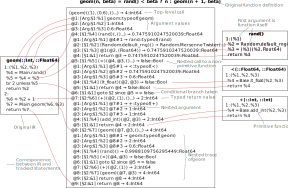
\includegraphics[width=\textwidth]{figures/wengert-list}
  \caption{Extended Wengert list for one run of the stochastic function geom (only three levels
    shown). The central box is the tracked graph of the call \protect\jlinl{geom(1, 0.6)}. The other
    boxes show the original IR of the called non-primitive functions, to which the nodes are
    linked.  Angle brackets indictate constant values.}
  \label{fig:ext-wengert-list}
\end{figure}

Figure~\ref{fig:ext-wengert-list} illustrates the resulting extended Wengert list for one run of a
short stochastic function:
\begin{lstlisting}
geom(n, beta) = rand() < beta ? n : geom(n + 1, beta)
\end{lstlisting}
(for readability, recorded to only three levels of nesting).  The function draws a sample from the
geometric distribution with parameter \jlinl{beta}, starting to count at value \jlinl{n}. On the
left, we have its IR in textual form, consisting of two blocks. The central part is the graph of
nested nodes.  There, values and jumps from the top-level call are recorded in their encountered
order, as nodes with \enquote{tape references} \jlinl{@1} to \jlinl{@9}. SSA variables (\jlinl{\%i})
occurring in expressions of SSA definitions are also replaced in the nodes by the respective tape
references.  Each node is linked to the original IR statement it records, as indicated by the red
arrows.

In the lower middle part, we see the node corresponding to the statement \jlinl{\%7 = geom(\%6,
  \%3)}.  It is recorded at reference \jlinl{@8} with expression \jlinl{geom(@7, @3)} and value
\jlinl{4} (the notation \jlinl{⟨geom⟩(@7, @3, ()...)} indicates that \jlinl{geom} is a constant, and
no variadic arguments are passed). The values of the arguments of this call can be inspected by
looking up the respective references.  Since \jlinl{geom} is not a primitive function, the node
holds tape of child nodes as well.  In this case, it is equivalent to the top level, due to the
recursivity of \jlinl{geom}. We can see the three arguments \jlinl{@1}, \jlinl{@2}, and \jlinl{@3},
corresponding to the block arguments \jlinl{\%1}, \jlinl{\%2}, and \jlinl{\%3}, with the value of
\jlinl{@2} being now \jlinl{2} instead of \jlinl{1}.  Further we can see function calls of
\jlinl{rand} and \jlinl{<} as well as a conditional jump, corresponding to the branch the original
IR, followed by calls of \jlinl{+} and \jlinl{geom}. Following back the tape references from the
result value \jlinl{@9}, the data path of the trace can be extracted.  It can be used for
reverse-mode AD, and only these nodes would be recorded in a conventional Wengert list.  In our
system, however, we also record the nodes on the control path, consisting of \jlinl{@6} and the
nodes it depends on.


\section{Automatic Graph Tracking}
\label{sec:autom-graph-track}

Recording an extended Wengert list requires to record all block arguments, SSA definitions, and
taken branches, with their actual values and metadata. This is achieved by extending the IR with new
statements creating nodes and recording them on the extended Wengert list structure described
above. Care needs to be taken to properly record function calls, since we need to ensure that
non-primitive functions are recursively tracked.   

The transformed code of the example function geom, whose IR is displayed in
figure~\ref{fig:ext-wengert-list} above, is displayed in listing~\ref{lst:geom-tracked}.  First, a
\enquote{graph recorder} object is set up in the extra argument \jlinl{\%5}.  In this, the original
IR is stored.  Subsequently, every statement is replaced by a call to one of the
\protect\jlinl{trackedX} functions, to which both the function and its arguments, wrapped into
\jlinl{TapeExpression}s directly (for constants) or indirectly (through \jlinl{trackedvariable} and
\jlinl{trackedargument}, which preserve the symbolic mapping to SSA variables).  The \jlinl{record!}
function takes care of constructing the child node of the possibly nested call, and storing them on
the recorder object.

Branches, tracked with \jlinl{trackejump} and \jlinl{trackedreturn}, cannot be stored on the
recorder object before they are taken, of course.  The solution is to first construct the respective
nodes of all possible branches of a block, and adding them as an extra argument to the branches
taken.  Then, in each target branch, the jump node from which the branch originated is recorded
immediately.  As a special case, all return branches are converted to unconditional jumps to one new
block at the end, which contains a single unified return statement.  This way, they can be treated
in the same way as other branches.

The resulting IR consists of about three to five times as many statements as the original.  The
transformation, due to JIT compilation, is performed at most once per method and then stored as
compiled code.  However, the tracking~-- the recording of all statements in the extended Wengert
list structure~-- happens at every execution during runtime.

\begin{lstfloat}[p]
  \hrule
  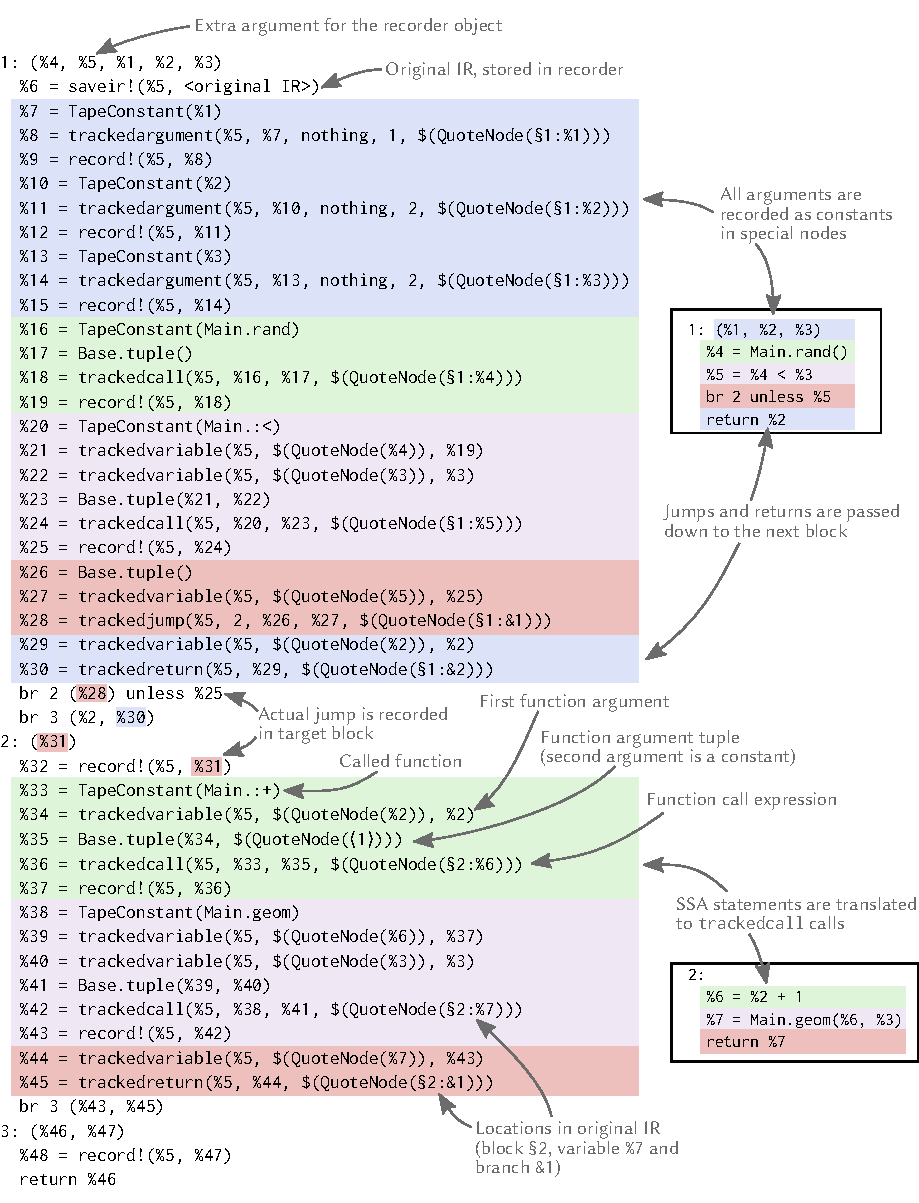
\includegraphics[width=\textwidth]{figures/translation}
  \hrule
  \caption{Tracked IR of the method \protect\jlinl{geom(::Int, ::Float64)}.  Parts corresponding to
    original IR are highlighted in matching colors.}
  \label{lst:geom-tracked}
\end{lstfloat}
\todo{make sure the figure in on same spread as explanation}

Please see the appendix for a pseudo-code specification of the IR transformation in Algorithm 1, and
the transformed code for the geom function in Figure 3.\todo{describe algorithm}

\begin{algorithm}[p]
  \hrule\footnotesize
  % \smallskip
  % This transformation happens inside a generated function called by \jlinl{trackcall}, which
  % assembles the resulting value and IR into a new node with the correct metadata.
  % \par\vspace{\baselineskip}
  % Missing from the description are the recording of metadata, the exact constructions of nodes, and
  % the mechanisms to correctly rename SSA variables during the transformation and tape references at
  % runtime.
  \begin{algorithmic}
    \State Initialize \jlinl{new_ir} \Comment create empty IR object
    \For{\jlinl{old_block} in \jlinl{blocks(ir)}}
    \State Add an empty block \jlinl{new_block} to \jlinl{new_ir}
    % 
    \If{\jlinl(arg) is the first block}
    \State Add variable \jlinl{\%recorder} to \jlinl{new_block}
    \EndIf
    %
    \For{\jlinl{arg} in \jlinl{arguments(old_block)}}
    \State Add \jlinl{arg} to \jlinl{new_block}
    \EndFor
    %
    \If{there exist branches to \jlinl{old_block}}
    \State Add argument \jlinl{\%branch_node} to \jlinl{new_block}
    \State Add statement to \jlinl{new_block}, recording \jlinl{\%branch_node} in \jlinl{\%recorder}
    \EndIf
    %
    \For{\jlinl{arg} in \jlinl{arguments(old_block)}}
    \State Add statement \jlinl{\%node} to \jlinl{new_block}, creating a node for \jlinl{arg}
    \State Add statement to \jlinl{new_block}, recording \jlinl{\%branch_node} in \jlinl{\%recorder}
    \EndFor
    %
    \For{\jlinl{stmt} in \jlinl{statements(old_block)}}
    \If{\jlinl{stmt} is a normal call}
    \State Add statement \jlinl{\%call_node} to \jlinl{new_block}, calling \jlinl{trackcall} on \jlinl{stmt}
    \State Add statement to \jlinl{new_block}, recording \jlinl{\%call_node} in \jlinl{\%recorder}
    \ElsIf{\jlinl{stmt} is a \enquote{special} call or constant}
    \State Add statement \jlinl{\%node} to \jlinl{new_block}, creating a node for \jlinl{stmt}
    \State Add statement to \jlinl{new_block}, recording \jlinl{\%node} in \jlinl{\%recorder}
    \EndIf
    \EndFor
    %
    \For{\jlinl{branch} in \jlinl{branches(old_block)}}
    \If{\jlinl{branch} is a return branch}
    \LineComment{Substitute return by a branch to the \enquote{return block}}
    \State Add statement \jlinl{\%return_node} to \jlinl{new_block}, creating a return node
    corresponding to \jlinl{branch}
    \State Add branch to \jlinl{new_block}, targeting the return block, copying \jlinl{branch}'s
    argument, with \jlinl{\%return_node} as extra argument
    \Else
    \State Add statement \jlinl{\%branch_node} to \jlinl{new_block}, creating a node for \jlinl{branch}
    \State Add branch to \jlinl{new_block}, copying \jlinl{branch}, with \jlinl{\%branch_node} as
    extra argument
    \EndIf
    \EndFor
    \EndFor
    %
    \Statex
    \LineComment{Set up \enquote{return block}}
    \State Add block \jlinl{return_block} to \jlinl{new_ir}
    \State Add arguments \jlinl{\%return_value}, \jlinl{\%return_node} to \jlinl{return_block}
    \State Add statement to \jlinl{return_block}, recording \jlinl{\%return_node} in
    \jlinl{\%recorder}
    \State Add statement \jlinl{\%result} to \jlinl{return_block}, creating a tuple of
    \jlinl{\%return_value} and \jlinl{recorder}
    \State Add return to \jlinl{return_block}, returning \jlinl{\%result}
  \end{algorithmic}
  \smallskip
  \hrule
  \caption{IR transformation to record an extended Wengert list (simplified) \label{alg:ir-transform}}
\end{algorithm}




\section{Evaluation}
\label{sec:irtracker-eval}

%%% Local Variables: 
%%% TeX-master: "main"
%%% End: